\chapter{Computación en BigData y Visualización de Datos}

En este capítulo se van ha explicar algunos temas más generales como el Big Data y la implicación que tiene en la sociedad, las herramientas utilizadas principalmente para gestionar tanta información guardada, y el proceso de adaptar las técnicas clásicas para generar diagramas al nuevo enfoque sobre Big Data.

\section{BigData}

En la actualidad, las grandes empresas del mundo gestionan grandes cantidades de información. Cuando se define que cantidad de datos va relacionada con \textit{BigData}, se habla de terabytes, petabytes, o incluso, exabytes. Aparte del gran volumen de información, también es importante tener en cuenta la variedad de los datos, su estructura y procedencia, por ejemplo, redes sociales, telefonía móvil, geolocalización, etc. No solo se genera información entre personas y ordenadores, sino que la comunicación entre distintos dispositivos, para mantener todas las herramientas interconectadas, genera una inmensa cantidad de datos de gran valor \cite{BigDataIntro}. 

Por eso, surge la necesidad de controlar y gestionar toda esta información tan diversa a través de nuevas técnicas, ya que los procesos y herramientas tradicionales son incapaces de procesar y analizar esta gran cantidad de información. Cuando el simple hecho de aumentar la capacidad hardware de los servidores de almacenamiento es insuficiente, es necesario utilizar algoritmos capaces de realizar esta tarea de manera rápida, sencilla y precisa. Por eso, uno de los principales paradigmas de programación de la actualidad, capaz de procesas la información \textit{BigData}, es el conocido MapReduce. MapReduce es el algoritmo capaz de procesar esas grandes cantidades de datos, y las herramientas utilizadas en este proyecto que implementan dicho algoritmo han sido Hadoop y Spark, de las que se va a tratar con mayor profundidad en los apartados siguientes.

Además del algoritmo MapReduce, la visualización de los datos también es un enfoque importante para ayudar a Big Data a obtener una visión completa de los datos y descubrir sus valores. Tanto el análisis como la visualización de \textit{BigData} deben integrarse perfectamente para su correcto funcionamiento en distintas aplicaciones. La visualización representa datos de una forma sistemática que permite a las grandes empresas mezclar fuentes de datos dispares para crear vistas analíticas personalizadas \cite{BigDataVisualization}. La analítica visual en \textit{BigData} se enfrenta a una serie de retos que vienen definidos por la “Regla de las 4 V’s”. Los retos de las 4 V’s serían los siguientes \cite{OverviewBigDataVis}: 

\begin{itemize}
	\item Volumen: Los métodos se desarrollan para trabajar con grandes volúmenes de datos y permiten derivar el significado de grandes volúmenes de datos.
	\item Variedad: Los métodos se desarrollan para combinar tantas fuentes de datos como sea necesario (estructurados y no estructurados).
	\item Velocidad: Con los métodos de visualización, las empresas pueden reemplazar los procesos batch por procesamiento en tiempo real.
	\item Valor: los métodos no sólo permiten a los usuarios crear infogramas llamativos, sino también aumentar el valor de negocio mediante la obtención de conocimientos a partir de \textit{BigData}.
\end{itemize}

\section{MapReduce}

El paradigma MapReduce es un modelo de programación enfocado en resolver los problemas de computación de grandes cantidades de datos, de manera paralela y distribuida. Este estilo de programación se creó inspirado en dos funciones de programación funcional: Map y Reduce. El objetivo de MapReduce es resolver problemas con conjunto de datos muy grandes, y por eso, se centra en la paralelización de los cálculos. 

\begin{figure}
	\centering
	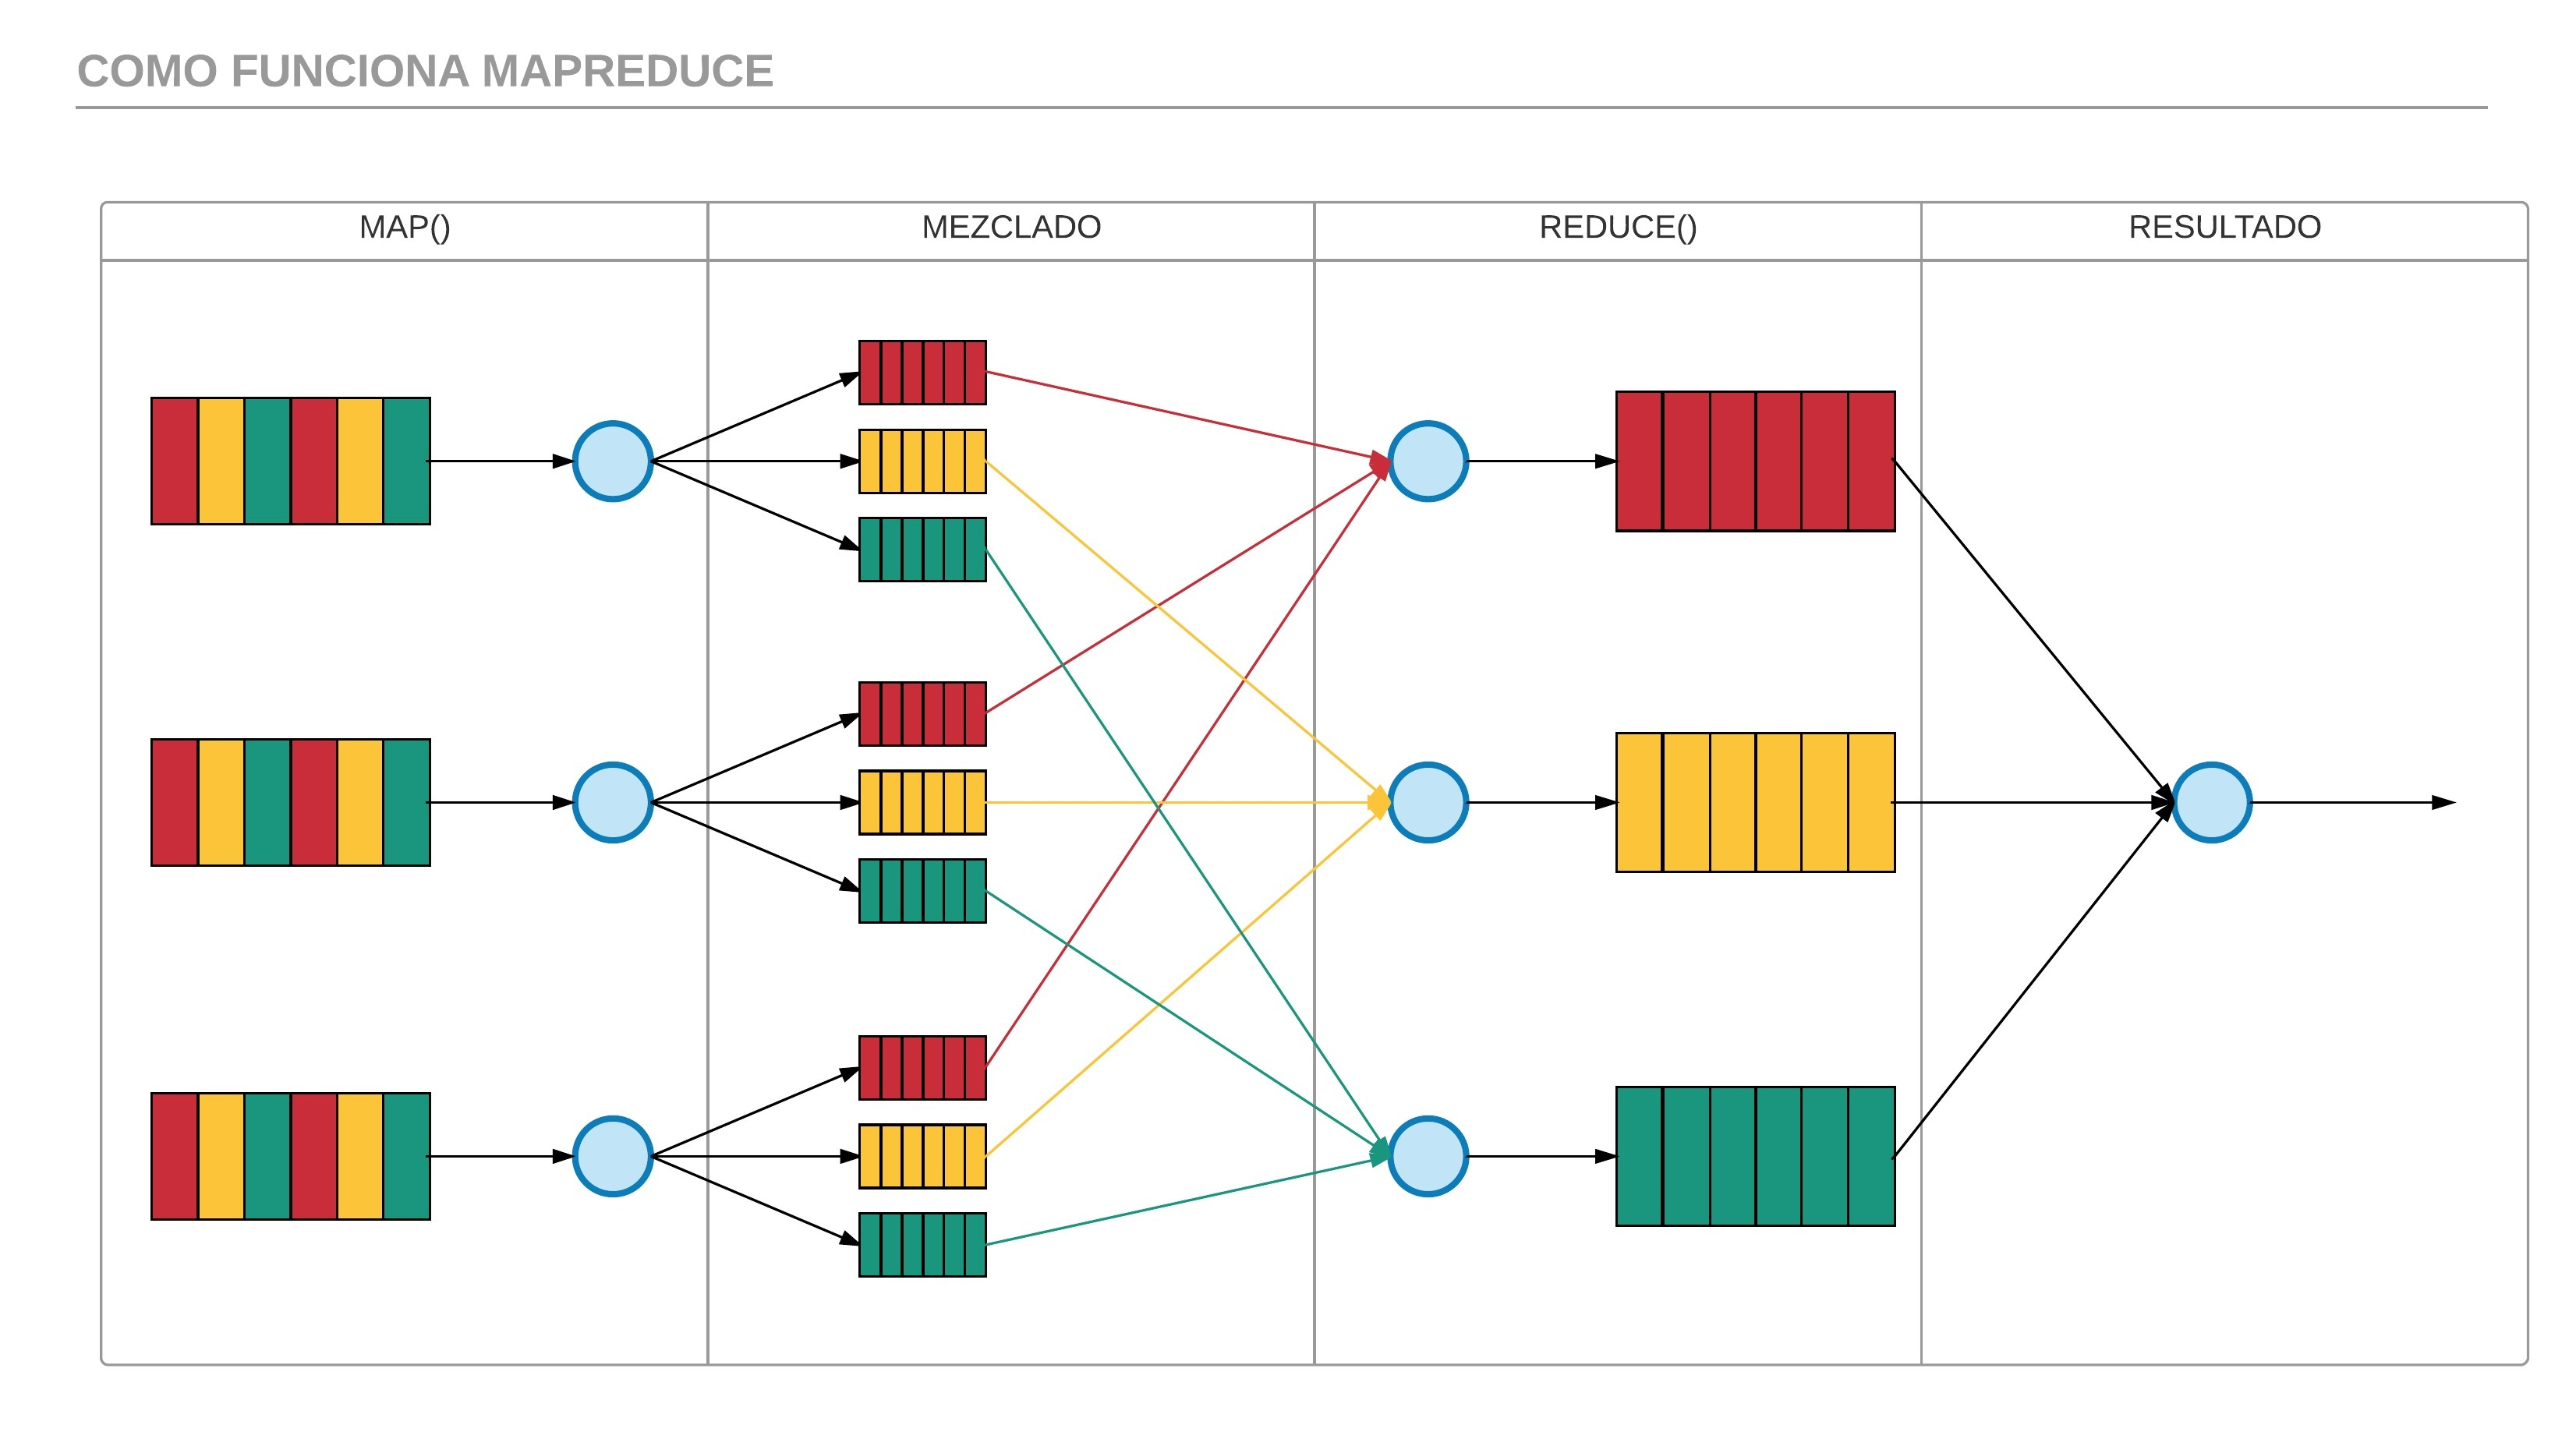
\includegraphics[width=1\linewidth]{imagenes/Como_funciona_MapReduce}
	\caption{Funcionamiento de MapReduce}
	\label{fig:comofuncionamapreduce}
\end{figure}

Se puede explicar el funcionamiento de MapReduce como una división del cálculo en distintas fases, como se aprecia gráficamente en la figura \ref{fig:comofuncionamapreduce}.
Primero una fase de mapeo o transformación de datos, la cual se encarga de aplicar una función de cómputo sobre los mismos, manteniéndose dentro de la misma fase el resultado del procesamiento. Este resultado no se almacena en el momento de ejecutar la función, sino que se acumulan todas las transformaciones hasta la segunda fase. En esta segunda fase se realizan las llamadas acciones o funciones de reducción, que se encargan de calcular un resumen de los datos, como puede ser una sumatoria, como se muestra en la figura \ref{fig:flujodedatosenmapreduce}.

\begin{figure}
	\centering
	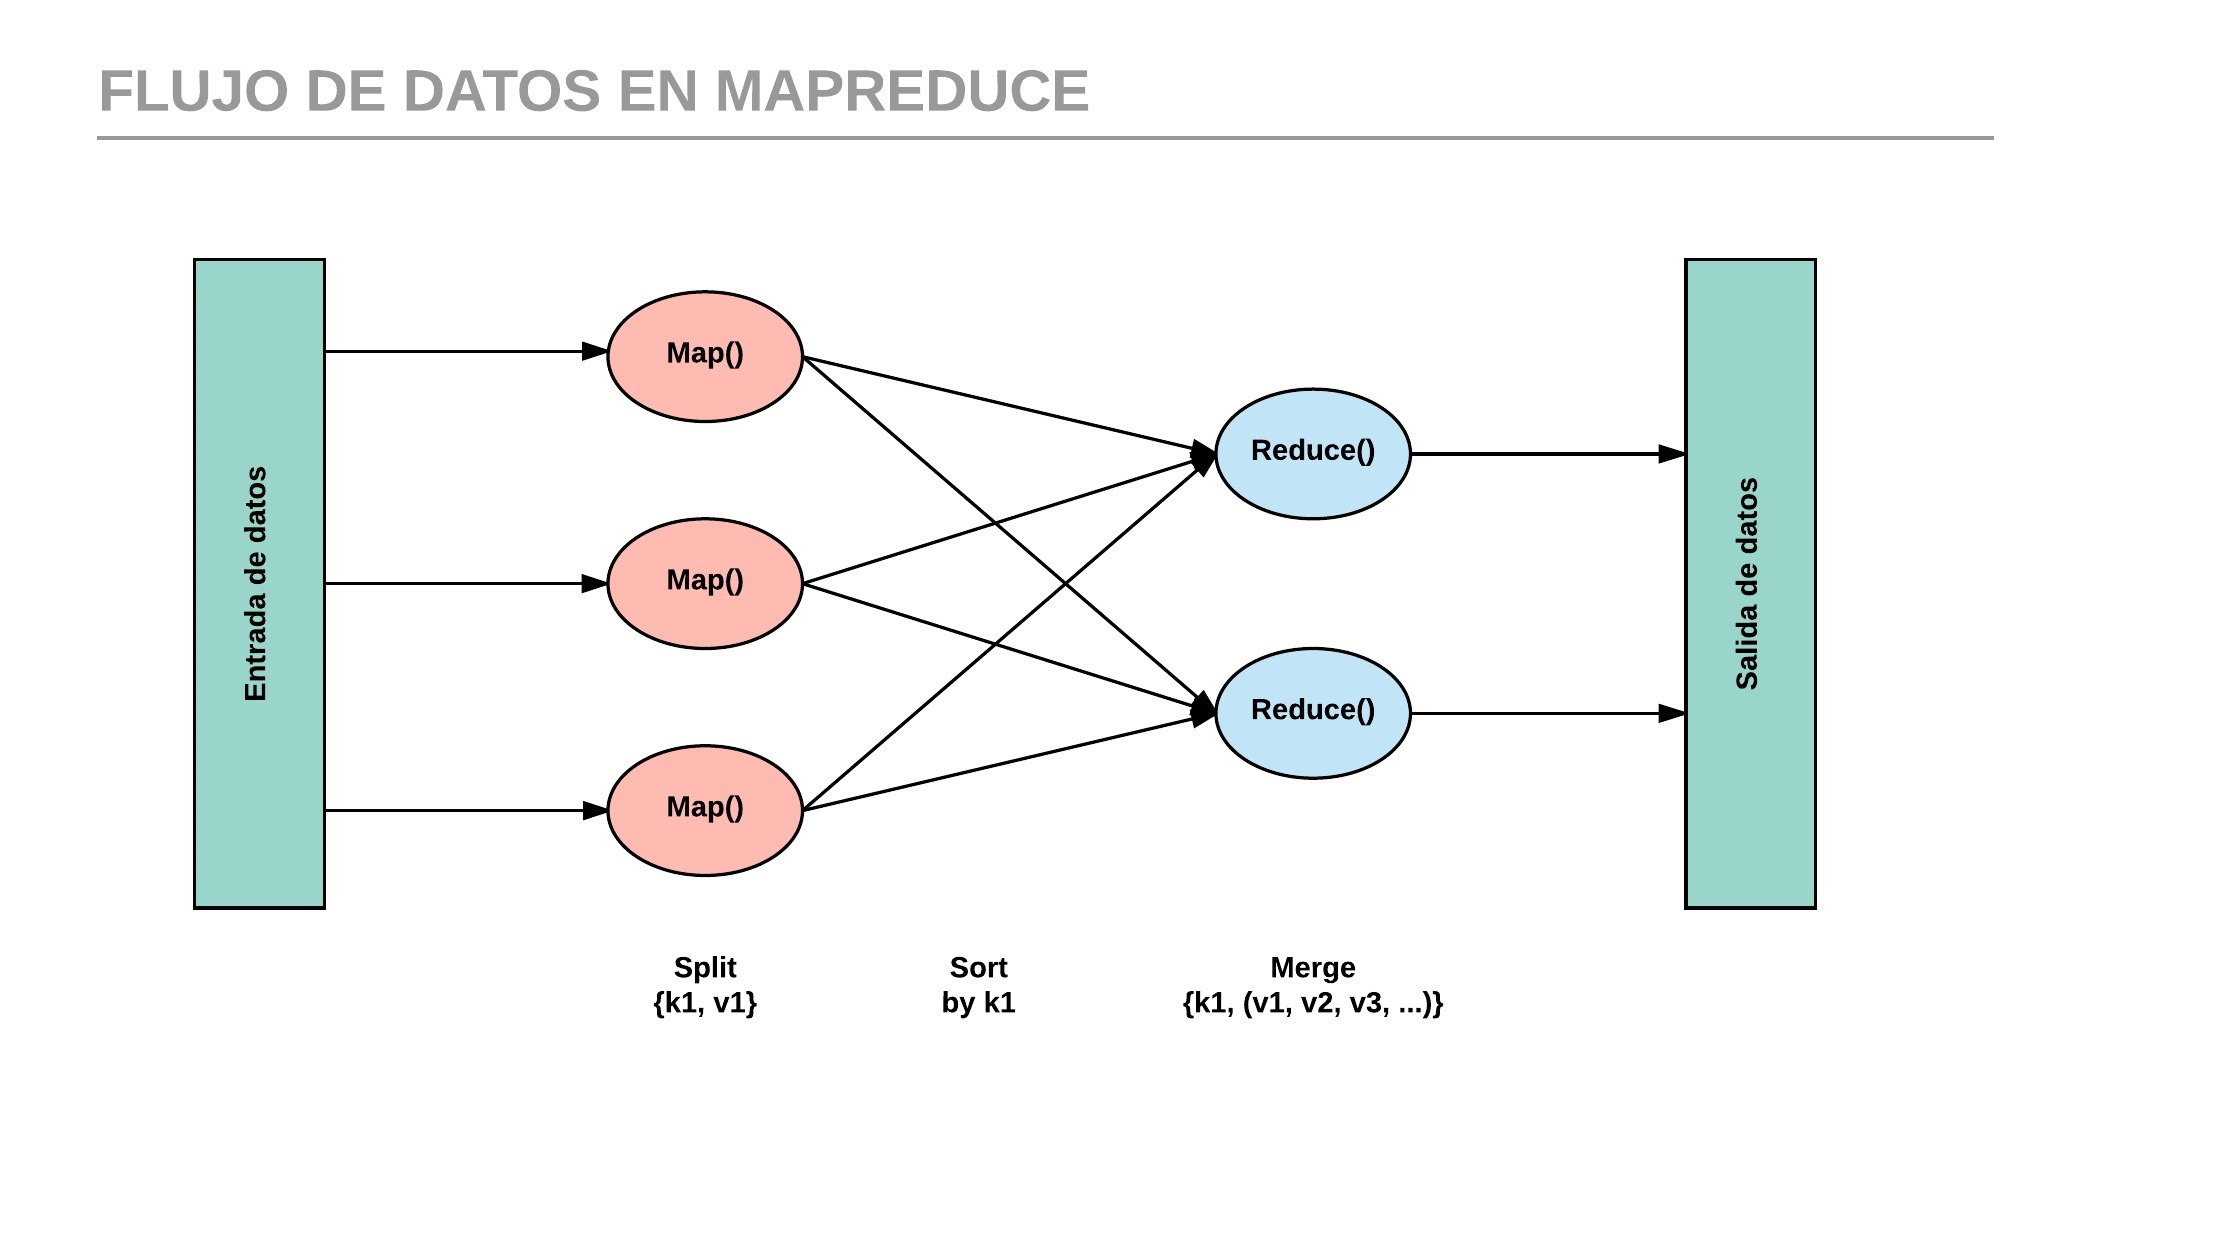
\includegraphics[width=1\linewidth]{imagenes/Flujo_de_datos_en_MapReduce}
	\caption{Flujo de datos en MapReduce}
	\label{fig:flujodedatosenmapreduce}
\end{figure}

En cada una de las fases se elige una o varias funciones correspondientes de la misma. Los datos se adaptan a una estructura ‘key-value’ para poder subdividir una tarea entre los distintos recursos disponibles \cite{MRHadoopLibro}. 

\section{Hadoop}
\begin{minipage}{\textwidth}
	\centering
	
\includegraphics[width=0.4\textwidth]{imagenes/hadoop_logo.png}\\[0.1cm]
\end{minipage}

\textbf{Apache Hadoop} \cite{HadoopInicial} es un entorno de trabajo Open-Source que ofrece computación escalable y distribuida, sobre grandes conjuntos de datos. Hadoop permite la escalabilidad desde un servidor, hasta cientos de ellos, solamente ajustando unos pocos parámetros \cite{HadoopInicial}. Este framework ofrece una amplia gama de funcionalidad gracias a tres grandes cualidades que posee:
\begin{itemize}
	\item La escalabilidad, permitiendo guardar y distribuir enormes conjuntos de datos en cientos de servidores que funcionan en paralelo. 
	\item La flexibilidad que ofrece con respecto al tipo de datos que almacena, es una de las grandes ventajas del sistema, ya que no importa el tipo de fichero que se quiere guardar o la fuente de la que provienen. 
	\item Su tolerancia a fallos lo hace uno de los más robustos del mercado, ya que el propio sistema siempre mantiene copias de los datos en los distintos nodos de los clusters, permitiendo la posibilidad de recuperarse en caso de errores.	
\end{itemize}

La estructura de Hadoop está basada en cuatro grandes módulos, que se detallan a continuación:
\begin{itemize}
	\item Hadoop Common: Este módulo es la base de Hadoop. Proporciona los ficheros fuente del sistema, necesarios para su ejecución sobre los cluster. También proporciona la documentación necesaria para la instalación y ejecución.
	\item Hadoop Distributed File System (HDFS): Se trata de un sistema de archivos que permite acceder a los datos guardados en el servidor. Tiene un gran nivel de abstracción, lo que permite acceder a los archivos de datos de manera fácil, sin la necesidad de conocer la ubicación real, es decir, en que cluster se encuentran los datos. Es tal abstracción, que si los ficheros están fraccionados y ubicados en distintas localizaciones internamente, seguiría visualizándose como un único archivo y procesándose como tal.
	
	La estructura HDFS se divide en dos conceptos clave, un ‘Namenode’ y múltiples ‘Datanode’. Este concepto se basa en la estructura clásica maestro-esclavo, donde el Namenode sería la de maestro, cuya función es gestionar el espacio de nombres del sistema de archivos y controlar el acceso por parte de los clientes a los archivos. Los Datanodes, por el contrario, son la parte esclava de la estructura. Suele haber uno por cluster en el servidor donde se ejecuta HDFS. 
	La función de esta estructura es dividir los ficheros de datos en varios bloques, que se almacenan en los distintos Datanodes, replicando algunos de estos mismos bloques en varios Datanodes para ofrecer una tolerancia a fallos mayor. En el caso del Namenode, se encarga de dirigir que Datanode almacena cada parte del archivo, teniendo siempre constancia de cada una de la ubicación.
	
	Por parte del cliente, permite realizar operaciones como abrir, modificar, borrar archivos, etc, sin la necesidad de conocer la localización del mismo \cite{HDFSHadoopLibro}.  Se puede apreciar, de manera más gráfica, el sistema HDFS en la figura \ref{fig:hdfsestructura}.
	\item Hadoop YARN: Es un framework que permite gestionar los recursos disponibles para la instalación y ejecución de Hadoop. Se trata de una herramienta para gestionar los clusters disponibles, configurar el comportamiento de cada uno de ellos, y poder balancear la carga de trabajo de cada uno de ellos. Suele utilizarse una estructura Maestro-Esclavo en los sistemas Hadoop.
	\item Hadoop MapReduce: La base de Hadoop es el paradigma MapReduce, explicado anteriormente. Está orientado a resolver problemas con grandes conjuntos de datos, por lo que utiliza el sistema de archivos distribuido (HDFS).
\end{itemize}

\begin{figure}
	\centering
	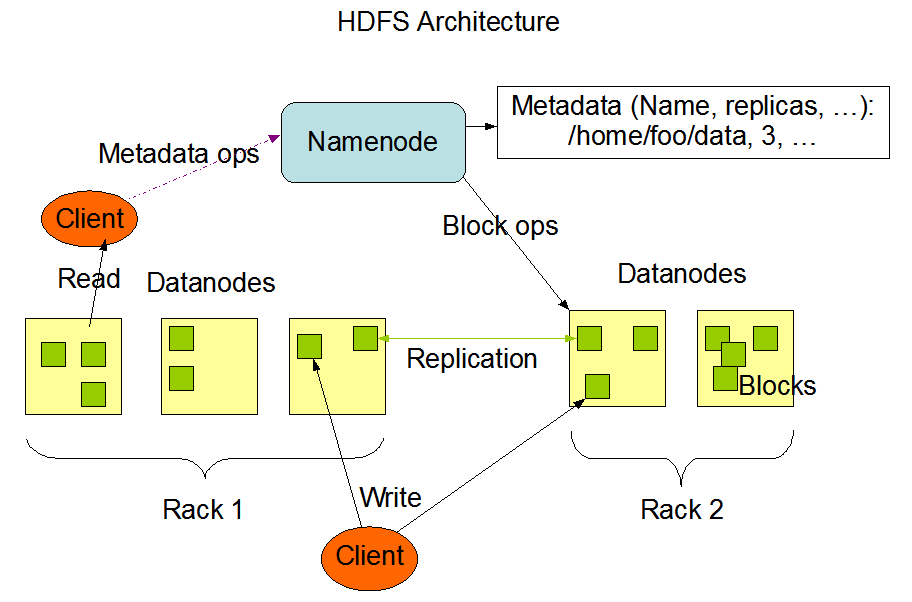
\includegraphics[width=1\linewidth]{imagenes/hdfs_estructura}
	\caption{Arquitectura del HDFS \cite{HadoopHDFS}}
	\label{fig:hdfsestructura}
\end{figure}

En la API, la idea de usar Hadoop es como almacenamiento y gestión de los ficheros de datos, gracias a las ventajas que ofrece para detectar y gestionar fallos. Otra de las grandes ventajas es su fácil y precisa conexión con la herramienta Apache Spark. Esta nueva herramienta, permite suprimir algunas de las carencias de Hadoop, como por ejemplo, tener una API sencilla con la que trabajar en lenguajes como Scala (su lenguaje nativo), Java, Python o SparkSQL. Otra de las debilidades de Hadoop es su rendimiento, ya que todos los datos están en disco, pero Spark cubre esta carencia pudiendo trabajar en memoria. Como resultado de esto, todos los cálculos se aceleran considerablemente, y hablando de grandes volúmenes de datos, es imprescindible la rapidez. 
En la siguiente sección, se explica con detalle la funcionalidad de Spark.

\section{Spark}

\begin{minipage}{\textwidth}
	\centering
	
\includegraphics[width=0.3\textwidth]{imagenes/spark_logo.png}\\[0.1cm]
\end{minipage}

\textbf{Apache Spark} \cite{SparkInicial} es un entorno de trabajo Open-Soruce diseñador para procesar grandes cantidades de datos de una manera sencilla, rápida y con grandes capacidades de analítica. En los últimos años, se ha alzado como un referente en la computación de Big Data, al solucionar algunas carencias que tiene Hadoop, y mejorar otros aspectos fundamentales. Principalmente, mejora el paradigma MapReduce haciéndolo más rápido y con procesamiento de datos en tiempo real, gracias al cómputo de los mismos en memoria \cite{SparkInicial}.

Una de las grandes ventajas de Spark es su soporte para compilar código en varios lenguajes, como Scala, Java, Python o R. Esto confiere a la herramienta una gran versatilidad cuando se trabaja con ella.

Las aplicaciones diseñadas en Spark se ejecutan como conjuntos independientes de procesos sobre un cluster. El encargado de coordinar estos procesos es el objeto SparkContext \cite{SparkClusterOverview}.

Para ejecutarse en un cluster, el objeto SparkContext se conecta a los gestores de cada uno de los clusters, como por ejemplo Spark Mesos o YARN. Estos son los encargados de asignar los recursos disponibles entre las aplicaciones. Una vez ejecutado, Spark obtiene el control de los procesos ejecutores, encargados de gestionar los cálculos y el almacenamiento de datos de la aplicación. Por último, Spark envía el código de la aplicación (contenido en archivos JAR o Python controlados por SparkContext) a los ejecutores, para que estos lo ejecuten.

Cada una de las aplicaciones que se ejecutan en Spark, tienen su propio proceso ejecutor. Esto quiere decir, que son independientes entre sí, tanto en el lado de la programación como en el ejecutor. Están completamente aisladas, por lo que cada una tiene sus propios recursos del sistema. Sin embargo, esto significa también que no se comparten los datos entre las distintas instancias de los objetos SparkContext, a menos que estén localizados en un sistema de almacenamiento externo a Spark. 

\begin{figure}
	\centering
	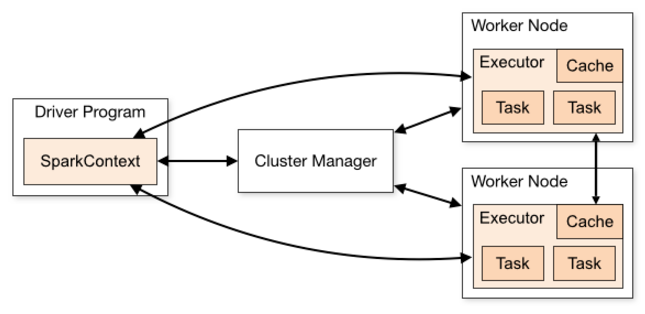
\includegraphics[width=1\linewidth]{imagenes/spark_estructura}
	\caption{Estructura del funcionamiento interno de Spark \cite{SparkClusterOverview}}
	\label{fig:sparkestructura}
\end{figure}

En un nivel de abstracción alto, cada una de las aplicaciones de Spark consiste en un programa controlador, que ejecuta el código diseñado por el usuario, encargándose el propio Spark de dividir y ejecutar las funciones paralelas dentro del mismo código sobre el cluster.
La principal abstracción que proporciona Spark es el conocido RDD (Resilient Distributed Dataset) \cite{SparkRDD}. RDD es una colección de elementos divididos a través de los nodos del cluster que pueden funcionar en paralelo. Una de las maneras de crear un RDD es con un archivo dentro del sistema de archivos de Hadoop (HDFS), por ejemplo. La recuperación automática que ofrece un RDD ante fallos en los nodos, es una de las grandes características que tienen. 

Otra característica de Spark son sus variables compartidas entre las funciones que se ejecutan en paralelo. Cuando se ejecutan estas funciones, Spark envía una copia de todas las variables utilizadas en la función a cada una de las tareas, ya que a veces una variable necesita ser compartida entre distintas tareas, o entre las tareas y el programa administrador. Hay dos tipos de variables compartidas distintas:
\begin{itemize}
	\item Variables de difusión: Se utilizan para almacenar en caché un valor compartido en todos los nodos.
	\item Acumuladores: Se utilizan para guardar resultados de operaciones de tipo \textit{reduce}.
\end{itemize}

\begin{figure}
	\centering
	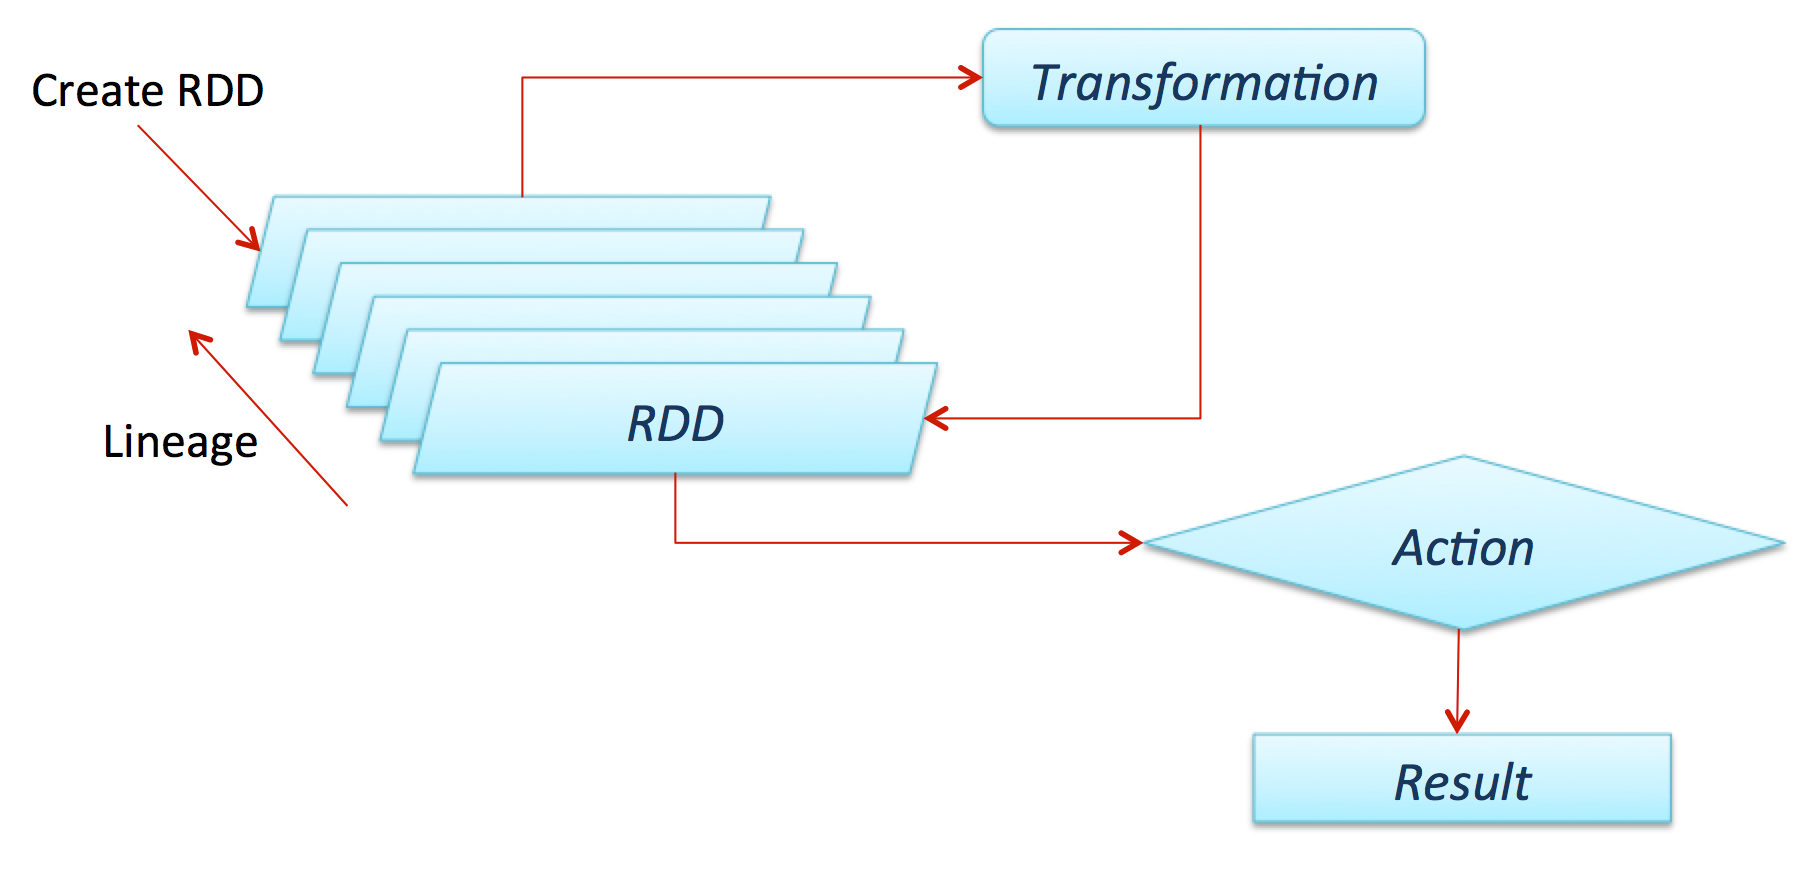
\includegraphics[width=1\linewidth]{imagenes/spark_rdd}
	\caption{Funcionamiento de un RDD \cite{SparkRDDFuncionamiento}}
	\label{fig:sparkrdd}
\end{figure}

La combinación de Hadoop y Spark, crea una potente herramienta para el cómputo y análisis de grandes cantidades de datos. En la API, la principal función de Spark es de conexión con los ficheros almacenados en cluster con HDFS, la aplicación de técnicas de reducción y agrupación de los mismos, y el cómputo de los datos para obtener un resultado que pueda ser interpretado y representado gráficamente.
Además, permite la ejecución paralela de varios procesos, dándole una potencialidad mayor a la API.

\section{MongoDB}
\begin{minipage}{\textwidth}
	\centering
	
\includegraphics[width=0.4\textwidth]{imagenes/mongoDB_logo.png}\\[0.1cm]
\end{minipage}

Antes de hablar de \textbf{MongoDB}, es necesario explicar que significa una base de datos NoSQL y de donde procede. La idea de una base de datos NoSQL nace de la necesidad de gestionar la gran cantidad de información que se genera a partir de la web 2.0. Las limitaciones de las bases de datos relacionales con respecto al volumen de datos o la escalabilidad de los mismos, hace de las NoSQL una solución eficiente.
La principal diferencia entre ambas es que las NoSQL no siguen el esquema ‘Entidad-Relación’ ni tampoco almacenan los datos en estructuras de tablas, sino que utilizan el formato ‘Key-Value’, mapeo de columnas o grafos \cite{MongoDBNoSQL}. 

En la actualidad, MongoDB es el referente mundial en bases de datos NoSQL \cite{MongoDBRanking}. Esto significa que en vez de basarse en tablas, explicado anteriormente, almacena los datos en documentos dinámicos conocidos como BSON, una mejora de la estructura de datos JSON pero con el añadido de que puede almacenar datos binarios. Esta estructura aporta escalabilidad sobre los datos y un gran rendimiento, al procesar los accesos de lectura y escritura en memoria \cite{MongoInicial}.

Su funcionalidad en la API es la de almacenamiento de los resultados obtenidos a través de Spark y el estado de los mismos. De esta manera, es más rápido y sencillo obtener los datos necesarios para la representación gráfica, permitiendo el lanzamiento y obtención, de manera paralela, de los mismos. 
La idea es mantener una base de datos con dos colecciones distintas, una que mantenga el estado actual de cada uno de los gráficos generados con la herramienta, generando un identificador cuando se solicite una petición de representar un gráfico. La otra colección es la que almacena los resultados proporcionados por Spark, que son necesarios para dibujar el gráfico seleccionado. Dentro de esta colección, se usará el identificador generado anteriormente para conocer qué resultado de todos los almacenados es el que se ha solicitado.

\section{Visualización de Datos}

Llegar a entender que ocurre con los datos puede ser una tarea realmente costosa y muy difícil. Por esta razón, es necesario convertirlos a otro tipo de información, en este caso visual, para facilitar su comprensión. A parte de obtener las visualizaciones, es necesario tener el conocimiento de interpretarlas y tener la habilidad de aplicar los resultados obtenidos con un propósito final. 

La teoría es extrapolable a lo que se conoce como \textit{Big Data}, con la salvedad del problema que existe a la hora de almacenar, obtener, calcular e interpretar la inmensa cantidad de datos que pueden llegar a solicitarse para su visualización. Para lograr el objetivo de obtener el resultado de una forma rápida, sencilla y que sea accesible para todos en cualquier lugar, es necesario tener dos cuestiones en cuenta:
\begin{itemize}
	\item Hay que mantener la visualización perceptiblemente independiente del número de datos (de su volumen).
	\item Tener la posibilidad de interacción en tiempo real para el análisis exploratorio del conjunto de datos (de forma visual).
\end{itemize}

\subsection{Técnicas de reducción de datos}
La escalabilidad tanto en la visualización e interactividad debería estar limitada por la resolución elegida y no por el número de registros (independencia del número de datos). Por consecuente, es necesario aplicar técnicas de reducción de datos que nos permitan obtener un resumen más manejable de los mismos, lo que es mejor para su representación. Se realiza un muestreo o filtrado de los datos con el objetivo de mostrar un subconjunto representativo de los datos. Esto tiene un problema fundamental y es que es posible que se pierdan o se desechen valores atípicos o valores interesantes, es decir, que se puede perder elementos interesantes en la visualización.

También se pueden agregar los datos. Por ejemplo, subdividiendo los rangos de datos en secciones discretas y luego visualizar el número de puntos del sector con un mapa de densidad. De esta manera, se hacen menos suposiciones sobre cómo será el conjunto de datos y ayuda a preservar los patrones generales y los outliers, si hubiese.

\subsection{Elección de esquema de agrupación}
Es necesario tener una idea más o menos clara del tamaño de los contenedores, es decir, de los segmentos de igual tamaño en que se subdivide el rango de los datos. Hay que saber que el límite natural para representar unos datos, es el número de píxeles de la pantalla (o realmente del espacio de visualización física: pantalla, web, etc.). Es decir, la limitación que existe en el número de segmentos o de divisiones va a ser como máximo el número de píxel de pantalla (o entorno, etc). Para obtener más detalle de los datos, será necesaria una implementación interactiva del gráfico, que permita ampliar zonas concretas para profundizar en la información que representa.

\subsection{Agregación de los datos}
Una vez decidido los segmentos, es decir, el tamaño de los contenedores para los grupos de datos, es necesario realizar una operación de agregado para crear un resumen de esos datos en los contenedores. El agregado proporciona una forma de estimación de la densidad dentro de los límites del contenedor. Para ello, se pueden utilizar múltiples funciones como por ejemplo la media, la suma, el máximo, el mínimo, la moda etc. y otras funciones más complejas que suavizan la unión de contenedores contiguos.

\subsection{Suavizado de los datos}
También es posible realizar un suavizado de los datos, por ejemplo, una convolución con un kernel (matriz que representa el filtro, se aplica la convolución a cada pixel/dato centrado en el punto central, etc.), y se podría obtener una mejor aproximación con una serie de datos continuos. Sin embargo, este método puede tener un riesgo de concentración o valores atípicos de interés al realizar la evaluación de calidad de los datos.

\subsection{Visualizado de los datos}
Para la visualización de gráficos de datos masivos se recomienda el uso de principios de percepción (cómo se ven los plots) por ejemplo, para datos dimensionales. Cuando se tratan plots de una dimensión (1D, como histograma) podemos utilizar un eje para presentar y otro eje para representar los valores agregados. Para los datos en dos dimensiones (2D), se dificulta la representación. Para ello, se puede utilizar hasta los dos ejes simplemente mostrando los contenedores, pero para mostrar los cómputos globales se requiere utilizar una variable de codificación visual diferente como, por ejemplo, el tamaño o el color.

Las visualizaciones pueden ser estáticas o dinámicas. Las visualizaciones interactivas a menudo permiten hacer descubrimientos y un mejor trabajo que las herramientas de datos estáticos. Las visualizaciones interactivas pueden ayudar a obtener un gran conocimiento de Big Data. Los gráficos interactivos y la unión entre enfoques de visualización y redes o herramientas basadas en la Web pueden facilitar el proceso científico. La visualización basada en la Web ayuda a obtener datos dinámicos apropiados y mantener las visualizaciones actualizadas.

La extensión de algunos enfoques de visualización convencionales para manejar Big Data está lejos de ser eficiente. Es necesario desarrollar nuevos métodos y herramientas de visualización de Big Data para diferentes aplicaciones. En este proyecto se presentan avances en la visualización de Big Data y se ha llevado a cabo un análisis SWOT de herramientas de visualización actual para visualización de Big Data. Esto ayudará a desarrollar nuevos métodos y herramientas para la visualización de Big Data. La analítica y la visualización Big Data pueden integrarse perfectamente para funcionar mejor con las aplicaciones de Big Data. La realidad virtual inmersiva (VR) es un nuevo y poderoso método para manejar la alta dimensionalidad y la abstracción. Esto facilitará enormemente la visualización de Big Data.


